\section{Les vents}

La loi de Buys-Ballot indique que quand on est face au vent, l'anticyclone est à gauche, et la dépression à droite, dans l'hémisphère nord (l'inverse dans l'hémisphère sud).
		\begin{figure}[H]
			\centering
			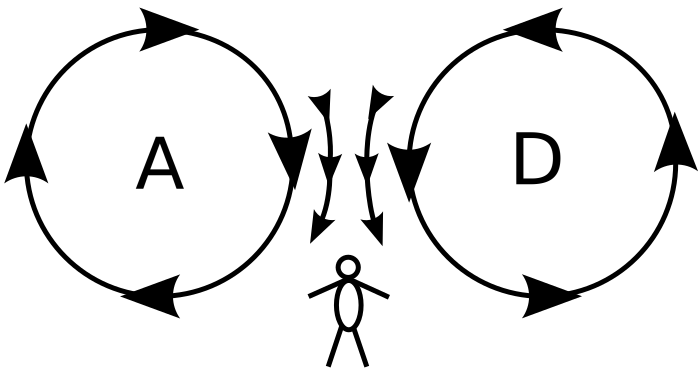
\includegraphics[width=0.4\linewidth]{03-Meteo/img/buysBallot.pdf}
			\legende{Illustration de la loi de Buys-Ballot}{img:buysBallot}
		\end{figure}	
		
		\astuce{Pour s'en souvenir, dans l'hémisphère nord (le notre) : les A : f\textbf{a}ce au vent, \textbf{a}nticyclone à g\textbf{a}uche.}